% ACM SIGCOMM Computer Communication Review (CCR), short technical paper. Rules read on 2 Nov 2026 (ccronline.sigcomm.org/instructions-for-submission):
% 6 two-column pages excluding references; acmart sigconf (the class of the CCR sample of Schmid, ACM acmart v2.21), 9 pt, US Letter, no copyright block (nonacm); NOT anonymous (names, affiliations, e-mails on the first page);
% abstract about 100 words; PDF at most 4 MB; no simultaneous submission elsewhere; submission via sigcomm-ccr.hotcrp.com. Implicit deadlines 1 Mar / 1 Jun / 1 Sep / 1 Dec.
\documentclass[sigconf,9pt,nonacm]{acmart}
\settopmatter{printfolios=true}
\renewcommand\footnotetextcopyrightpermission[1]{}
\setcopyright{none}
\pagestyle{plain}
\usepackage{booktabs,array}
\usepackage{xcolor}
\usepackage{xspace}
\usepackage{tikz}
\usetikzlibrary{arrows.meta}
% generated by make_assets_short.py - do not edit
\newcommand{\NCfg}{13}
\newcommand{\NExact}{12}
\newcommand{\NTcp}{14{,}200}
\newcommand{\NStageA}{5{,}200}
\newcommand{\NineShare}{35}
\newcommand{\NModelDiff}{25}
\newcommand{\NStageB}{9{,}000}
\newcommand{\CMaeZero}{0.30}
\newcommand{\CMaxZero}{0.7}
\newcommand{\CWrongZero}{0}
\newcommand{\CMaeOne}{7.39}
\newcommand{\CMaxOne}{99.4}
\newcommand{\CWrongOne}{2}
\newcommand{\CMaeTwo}{14.45}
\newcommand{\CMaxTwo}{99.4}
\newcommand{\CWrongTwo}{4}
\newcommand{\CMaeThree}{21.50}
\newcommand{\CMaxThree}{99.4}
\newcommand{\CWrongThree}{6}
\newcommand{\CN}{28}
\newcommand{\DN}{80}
\newcommand{\DDiff}{10}
\newcommand{\DJoinedWrongDiff}{10}
\newcommand{\DEarlyWrongDiff}{0}
\newcommand{\DJoinedMae}{17.8}
\newcommand{\DEarlyMae}{5.5}
\newcommand{\DJoinedWrong}{14}
\newcommand{\DEarlyWrong}{4}
\newcommand{\DBothWrong}{4}
\newcommand{\EFitEcdsa}{10}
\newcommand{\EFitMlFourFour}{12}
\newcommand{\EFitMlSixFive}{15}
\newcommand{\ECtlN}{36}
\newcommand{\ECtlMax}{0.9}
\newcommand{\ECtlWrong}{0}
\newcommand{\EN}{72}
\newcommand{\RJoinedMae}{1.42}
\newcommand{\RJoinedMax}{98.8}
\newcommand{\RJoinedWrong}{2}
\newcommand{\RJoinedRest}{142}
\newcommand{\RN}{144}
\newcommand{\RJoinedRestMax}{0.85}
\newcommand{\REarlyMae}{0.54}
\newcommand{\REarlyMax}{0.8}
\newcommand{\REarlyWrong}{0}
\newcommand{\REarlyRest}{144}
\newcommand{\RaceN}{221}
\newcommand{\RaceMlN}{134}
\newcommand{\RaceThr}{0.049}
\newcommand{\RaceRight}{132}
\newcommand{\RaceBeforePct}{90}
\newcommand{\RaceTwoRight}{36}
\newcommand{\RaceTwoScored}{36}
\newcommand{\RaceTwoOosRight}{394}
\newcommand{\RaceTwoOosN}{399}
\newcommand{\MixFitExc}{13}
\newcommand{\MixPredExc}{15}
\newcommand{\MixN}{4}
\newcommand{\MixRight}{3}
\newcommand{\NineDefMaeBefore}{13.3}
\newcommand{\NineDefMaeAfter}{1.2}
\newcommand{\NineN}{48}
\newcommand{\NineRwndDefOk}{7}
\newcommand{\NineRwndDefTot}{20}
\newcommand{\NineRwndLargeOk}{16}
\newcommand{\NineRwndLargeTot}{20}
\newcommand{\GenCells}{240}
\newcommand{\GenRespMax}{16}
\newcommand{\GenRttLo}{5}
\newcommand{\GenRttHi}{100}
\newcommand{\GenRateLo}{10}
\newcommand{\GenRateHi}{100}
\newcommand{\GenMtuLo}{1\,280}
\newcommand{\GenMtuHi}{9\,000}
\newcommand{\GenWEcRttFive}{10}
\newcommand{\GenWMFourFourRttFive}{10}
\newcommand{\GenWMSixFiveRttFive}{10}
\newcommand{\GenWEcRttThirty}{10}
\newcommand{\GenWMFourFourRttThirty}{12}
\newcommand{\GenWMSixFiveRttThirty}{15}
\newcommand{\GenWEcSlowTen}{10}
\newcommand{\GenWMFourFourSlowTen}{10}
\newcommand{\GenWMSixFiveSlowTen}{10}
\newcommand{\GenWEcMtuLow}{10}
\newcommand{\GenWMFourFourMtuLow}{12}
\newcommand{\GenWMSixFiveMtuLow}{16}
\newcommand{\ServCells}{48}
\newcommand{\ServWindow}{10}
\newcommand{\ServWrong}{0}
\newcommand{\BkN}{664}
\newcommand{\BkDef}{235}
\newcommand{\BkAOne}{44}
\newcommand{\BkAPct}{23.0}
\newcommand{\BkBRight}{248}
\newcommand{\BkBPct}{57.8}
\newcommand{\NtkRight}{18}
\newcommand{\NtkCells}{18}
\newcommand{\NtkEffect}{7}
\newcommand{\NtkEffectOk}{7}
\newcommand{\HN}{331}
\newcommand{\HLate}{117}
\newcommand{\HEarly}{214}
\newcommand{\HLateSS}{117}
\newcommand{\HWaitMed}{13.7}
\newcommand{\HEarlySS}{19}
\newcommand{\HAOne}{6}
\newcommand{\HALate}{117}
\newcommand{\HAPct}{5.1}
\newcommand{\HEnqMed}{181.2}
\newcommand{\HPcapMed}{-0.073}
\newcommand{\PhAfter}{164}
\newcommand{\PhAfterSS}{164}
\newcommand{\PhBefore}{500}
\newcommand{\PhBeforeSS}{61}
\newcommand{\StN}{799}
\newcommand{\StPOneRight}{799}
\newcommand{\StPOneN}{799}
\newcommand{\StPOnePct}{100.0}
\newcommand{\StPTwoRight}{212}
\newcommand{\StPTwoN}{236}
\newcommand{\StPTwoPct}{89.8}
\newcommand{\StPThreeRight}{51}
\newcommand{\StPThreeN}{74}
\newcommand{\StPThreePct}{68.9}
\newcommand{\StPTwoBRight}{236}
\newcommand{\StPTwoBN}{236}
\newcommand{\StDeferred}{71}
\newcommand{\StDeferredN}{96}
\newcommand{\StLate}{204}
\newcommand{\StLateInflight}{179}
\newcommand{\StLateLimited}{182}
\newcommand{\StEarly}{595}
\newcommand{\StEarlyLimited}{13}
\newcommand{\StBeforeN}{570}
\newcommand{\StBeforePk}{1}
\newcommand{\StAfterN}{204}
\newcommand{\StAfterPk}{10}
\newcommand{\KerN}{288}
\newcommand{\KerBeforeN}{216}
\newcommand{\KerBeforeSS}{0}
\newcommand{\KerAfterN}{72}
\newcommand{\KerAfterSS}{47}
\newcommand{\KerRight}{274}
\newcommand{\KerPct}{95.1}
\newcommand{\KerWrong}{14}
\newcommand{\KerMissLo}{0.039}
\newcommand{\KerMissHi}{0.080}
\newcommand{\KerMissNear}{0.031}
\newcommand{\AblFixedMae}{2.30}
\newcommand{\AblFixedOff}{4}
\newcommand{\AblFixedN}{144}
\newcommand{\AblSlowMae}{1.42}
\newcommand{\AblSlowOff}{2}
\newcommand{\AblSlowN}{144}
\newcommand{\AblLinuxMae}{1.42}
\newcommand{\AblLinuxOff}{2}
\newcommand{\AblLinuxN}{144}
\newcommand{\AblJoinedMae}{1.42}
\newcommand{\AblJoinedOff}{2}
\newcommand{\AblJoinedN}{144}
\newcommand{\AblEarlyMae}{0.54}
\newcommand{\AblEarlyOff}{0}
\newcommand{\AblEarlyN}{144}
\newcommand{\AblCFixedMae}{25.04}
\newcommand{\AblCFixedOff}{7}
\newcommand{\AblCFixedN}{28}
\newcommand{\AblCSlowMae}{35.63}
\newcommand{\AblCSlowOff}{10}
\newcommand{\AblCSlowN}{28}
\newcommand{\AblCLinuxMae}{0.30}
\newcommand{\AblCLinuxOff}{0}
\newcommand{\AblCLinuxN}{28}
\newcommand{\OvTwoSame}{247}
\newcommand{\OvTwoAll}{252}
\newcommand{\OvThreeSame}{247}
\newcommand{\OvThreeAll}{252}
\newcommand{\OvFourSame}{236}
\newcommand{\OvFourAll}{252}
\newcommand{\GxBaseCWrong}{0}
\newcommand{\GxBaseCLoose}{4}
\newcommand{\GxBaseDisEarly}{0}
\newcommand{\GxBaseDisJoined}{10}
\newcommand{\GxBaseEarlyWrong}{4}
\newcommand{\GxBaseMet}{4}
\newcommand{\GxFourCWrong}{0}
\newcommand{\GxFourCLoose}{4}
\newcommand{\GxFourDisEarly}{0}
\newcommand{\GxFourDisJoined}{10}
\newcommand{\GxFourEarlyWrong}{4}
\newcommand{\GxFourMet}{4}
\newcommand{\GxThreeCWrong}{0}
\newcommand{\GxThreeCLoose}{4}
\newcommand{\GxThreeDisEarly}{0}
\newcommand{\GxThreeDisJoined}{10}
\newcommand{\GxThreeEarlyWrong}{4}
\newcommand{\GxThreeMet}{4}
\newcommand{\GxMaxDiff}{0.05}
\newcommand{\CiWinLo}{64.0}
\newcommand{\CiWinHi}{99.8}
\newcommand{\CiJoinedLo}{95.1}
\newcommand{\CiJoinedHi}{99.8}
\newcommand{\CiRaceLo}{94.7}
\newcommand{\CiRaceHi}{99.8}
\newcommand{\CiKerLo}{92.0}
\newcommand{\CiKerHi}{97.3}
\newcommand{\CiNtkEffLo}{59.0}
\newcommand{\CiNtkEffHi}{100.0}
\newcommand{\SignDP}{0.002}
\newcommand{\SignNtkP}{0.016}

\newcommand{\pending}[1]{{\color{red}\textit{[pending: #1]}}}
\newcommand{\ms}{\,ms\xspace}
\newcommand{\citeone}{\cite{paperone}}
\graphicspath{{../Latex/figures/}}
\hyphenation{OpenSSL ac-knowl-edg-ment}
\setlength{\emergencystretch}{2em}

\begin{document}
\title{How Linux Grows the TCP Window After a Short Flight, and What It Costs Post-Quantum TLS}
\author{Trong-Hieu Dinh}
\affiliation{\institution{Banking Academy of Vietnam}\city{Hanoi}\country{Vietnam}}
\email{hieudt@hvnh.edu.vn}
\author{Trong-Minh Hoang}
\authornote{Corresponding author.}
\affiliation{\institution{Posts and Telecommunications Institute of Technology}\city{Hanoi}\country{Vietnam}}
\email{hoangtrongminh@ptit.edu.vn}
\begin{abstract}
Post-quantum signatures push TLS flights past the initial TCP window, so a flight's cost depends on the window Linux grows after the previous one. On plain TCP that window follows a one-line rule, exact in \NExact\ of \NCfg\ configurations and, under loss, without retransmission: with an initial window of ten, five segments leave it at ten and six lift it to twelve. Pre-registered predictions refute a larger-window explanation of a model error, and an intervention shows that OpenSSL's session ticket, written separately, enlarges the server's window. The rule is Reno's and Cubic's; BBR differs. Five recommendations follow.
\end{abstract}
\begin{CCSXML}
<ccs2012>
<concept><concept_id>10003033.10003039.10003048</concept_id><concept_desc>Networks~Transport protocols</concept_desc><concept_significance>500</concept_significance></concept>
<concept><concept_id>10003033.10003079.10011704</concept_id><concept_desc>Networks~Network measurement</concept_desc><concept_significance>300</concept_significance></concept>
<concept><concept_id>10002978.10003014.10003015</concept_id><concept_desc>Security and privacy~Security protocols</concept_desc><concept_significance>300</concept_significance></concept>
</ccs2012>
\end{CCSXML}
\ccsdesc[500]{Networks~Transport protocols}
\ccsdesc[300]{Networks~Network measurement}
\makeatletter\g@addto@macro\@concepts{\linebreak}\makeatother % break before the second bullet of the CCS concepts
\ccsdesc[300]{Security and privacy~Security protocols}
\keywords{TLS 1.3, post-quantum cryptography, TCP congestion window, measurement, design guidance}
\maketitle

\section{Introduction}
A post-quantum signature is large: 3\,309 bytes for ML-DSA-65 against about 70 for ECDSA-P256, nearly fifty times. A certificate chain built from them no longer fits in the 10-segment initial window of Linux~\cite{rfc6928}, and a flight that overflows the window costs a round trip. Dukkipati et al.\ argued for that window from web latency~\cite{dukkipati2010} and R\"uth et al.\ measured it across the IPv4 address space~\cite{rueth2017}, but both concern the window a connection starts with. We study what comes after: how far the kernel grows the window after a short flight, which decides whether the next flight (a request that carries a client certificate, say) crosses it. How the TLS library splits a flight into writes matters too.

Measurements of post-quantum handshakes find them slower~\cite{paquin2020,sikeridis2020,sosnowski2023,kampanakis2024}, and the closest treat the window as a setting. Henrich et al.\ vary the initial window on real servers: data beyond it adds a round trip, a larger window removes it~\cite{henrich2025}. Chou and Cao see the time to first byte rise in steps as certificate chains cross the initial window and approximate later windows by doubling; their resumed times are dominated by process start-up~\cite{chou2026}. Anastasova and Kampanakis attribute a rise of 51\ms (33\%) at 50\ms RTT to a client chain that exceeds the client's initial window, a setting of 10 or 24 segments, and do not resume~\cite{anastasova2025}. The latest systems study counts the server's TCP segments of full handshakes (one run per condition) and the loss tail of OpenSSL~3.5, but follows neither the window grown between flights nor resumed connections~\cite{dubetskyy2026}. We found no direct measurement of the window after short flights in this context.

The rule is more delicate than it looks. RFC~5681 and RFC~7661 describe slow start and window validation~\cite{rfc5681,rfc7661}, and Linux lets the window grow to twice the largest number of packets in flight~\cite{linuxcwnd}. Whether a five-segment flight passes the boundary $2\times5=10$ is one inequality, and it decides a round trip. We met it through an error of our own model. A per-segment transport model validated against OpenSSL~3.5 transactions~\citeone\ was right to within 1\ms\ on \RJoinedRest\ of \RN\ resumed configurations (exact 95\% interval \CiJoinedLo--\CiJoinedHi\%; the largest error \RJoinedRestMax\ms) and wrong by a whole round trip on two, both ML-DSA-44 with a large request (by 99\ms at 100\ms RTT and by 29\ms at 30\ms). A flight's cost cannot be read from its size. We ask how Linux grows the window after a short flight, and why those two transactions paid a round trip less than the model charged.

Our contributions are (1)~a closed-form window rule for plain TCP, tested in \NCfg\ configurations on seven machine-kernel combinations and under packet loss; (2)~tests with predictions fixed in advance showing that OpenSSL's session ticket, as a separate write, grows the server's window through acknowledgments whose effect depends on when the kernel processes them, with the registered criteria that failed reported as failed; (3)~the same tests on three OpenSSL releases, on Go's \texttt{crypto/tls}, under BBR and with delayed acknowledgments; and (4)~five recommendations for budgeting flights.

\begin{figure}[t]
\centering
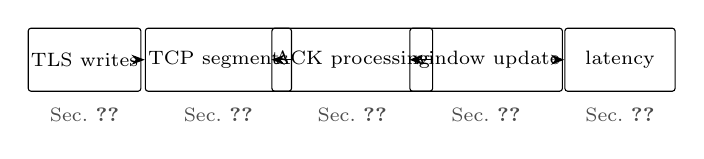
\begin{tikzpicture}[x=1mm,y=1mm,font=\scriptsize,>=Stealth,box/.style={draw,rounded corners=1pt,minimum width=14mm,minimum height=8mm,align=center,inner sep=1pt},note/.style={font=\scriptsize,text=black!70}]
\foreach \i/\t/\n in {0/TLS writes/{Sec.~\ref{sec:ticket}},1/TCP segments/{Sec.~\ref{sec:window}},2/ACK processing/{Sec.~\ref{sec:ticket}},3/window update/{Sec.~\ref{sec:window}},4/latency/{Sec.~\ref{sec:other}}}{
  \node[box] (b\i) at (\i*17,0) {\t}; \node[note] at (\i*17,-7) {\n};}
\foreach \i/\j in {0/1,1/2,2/3,3/4}{\draw[->] (b\i.east) -- (b\j.west);}
\end{tikzpicture}
\caption{From a TLS write to the latency of a transaction, and where the paper treats each step.}
\label{fig:overview}
\end{figure}

\section{Method}
The testbed is two network namespaces joined by a virtual link and shaped with \texttt{tc netem}. The main platform is an Intel i7-5600U under Linux 7.0.0-42 with OpenSSL~3.5; Section~\ref{sec:repl} repeats the tests elsewhere. TCP runs over IPv6 without timestamps (MSS = MTU$-60$), with Reno, and acknowledgments go out at once (\texttt{quickack} routes) unless stated. ``Window'' means the sender's congestion window (\texttt{snd\_cwnd}, in segments) unless we say receive window.

\emph{Plain TCP.} Each measurement starts a fresh connection. It writes $n_1$ full segments, waits for a 100-byte reply that acknowledges them all, reads the window from \texttt{TCP\_INFO}, and then times a second flight of $n_2$ segments, preceded by an 80-byte write like a TLS Finished. Stage~A reads the window after $n_1=1\ldots16,20,24,31,40$ in \NCfg\ configurations that change one factor at a time: RTT 5--100\ms; 10\,Mbit/s--1\,Gbit/s; MTU 1\,280, 1\,500, 9\,000; initial window 4, 10, 20; delayed ACK; Cubic; timestamps; offload (\NStageA\ connections). Stage~B times second flights in six configurations (\NStageB\ connections).

\emph{TLS with fixed predictions.} The TLS tests use resumed TLS~1.3 with mutual authentication, RTT 100\ms and 30 transactions per cell. Four suites (ECDSA-P256, ML-DSA-44, -65, -87) give ClientHellos of 2, 5, 6 and 8 segments, since the ClientHello carries the ticket and with it the client certificate. We committed the model's prediction for every cell, under every rule compared, before the measurement. Table~\ref{tab:tests} lists each test with its criterion and outcome: rows 1--5 count the cells wrong by a round trip ($>$50\ms at 100\ms RTT), rows 6--19 give a share or a count against the registered criterion. The archive lists the commit times of the predictions and of the first results, with checksums (\texttt{PREREGISTRATION\_L1.md}). They are git's own times, not an independent timestamp, and for the kernel and state traces only the analysis scripts with their thresholds preceded the run. Within a cell the interquartile range of the latency has a median of \SpreadMed\ms (at most \SpreadMax\ms) in the ticket-timing and client-window cells, against steps of one RTT: 30 transactions give a stable median but say nothing about tails.

\section{The Window After a Short Flight}\label{sec:window}
The window after an $n$-segment flight is
\begin{equation}
w(n)=\max\bigl(w_0,\;\min(w_0+n,\;2n)\bigr),
\end{equation}
exactly in \NExact\ of \NCfg\ configurations (exact 95\% interval \CiWinLo--\CiWinHi\%; Fig.~\ref{fig:window}). The configurations change one factor at a time and are not independent samples, so the interval is only descriptive. In words, nothing grows below $n=w_0/2$; the window is $2n$ for $w_0/2\le n\le w_0$; beyond $w_0$, every acknowledged segment adds one. Fig.~\ref{fig:window} shows medians of 20 connections against (1) (solid lines) and its two limits, $2n$ and $w_0+n$ for $w_0=10$ (dotted).

Three kernel functions produce this (mainline, checked 18 November 2026). With one acknowledgment per segment, \texttt{tcp\_\allowbreak reno\_\allowbreak cong\_\allowbreak avoid} returns at once unless \texttt{tcp\_\allowbreak is\_\allowbreak cwnd\_\allowbreak limited} holds, and only then does \texttt{tcp\_\allowbreak slow\_\allowbreak start} add the segments acknowledged. The test holds if the sender was window-limited when it sent (\texttt{is\_\allowbreak cwnd\_\allowbreak limited}, set by \texttt{tcp\_\allowbreak cwnd\_\allowbreak validate} when the flight fills the window), or, in slow start, while $\texttt{snd\_\allowbreak cwnd}<2\,\texttt{max\_\allowbreak packets\_\allowbreak out}$: twice the segments in flight, not twice the window. A flight of $n\ge w_0$ segments fills the window, so each of its $n$ acknowledgments adds one and the window becomes $w_0+n$. A shorter flight leaves the window unfilled with $n$ in flight. The window then grows by one until it reaches $2n$, and not at all if $w_0\ge 2n$.

A short program that applies this logic reproduces (1) for all 480 pairs of $w_0\in\{2,4,10,16,20,32\}$ and $n\le 80$, and the measured window at every point of the window scan except at MTU 9\,000 (\texttt{Simulation/window\_\allowbreak from\_\allowbreak kernel.py}). The rule holds for every tested RTT, rate, MTU 1\,280 and 1\,500, initial window ($w_0$ in (1)), delayed ACK, Cubic, timestamps and offload, and on every platform of Table~\ref{tab:repl}. At MTU~9\,000 it falls short (\NineShare\% of flights match), for a reason that follows from the same logic: the default receive buffer limits the sender to about seven segments of 8\,940 bytes, so the receiver's window stops it before its own does, \texttt{is\_\allowbreak cwnd\_\allowbreak limited} stays false and the window does not grow. With \texttt{tcp\_rmem} raised to 1\,MiB, \NineRwndLargeOk\ of \NineRwndLargeTot\ flight sizes follow (1), against \NineRwndDefOk\ by default; the other four (8 to 11 segments) stay one or two segments below it, unexplained.

What matters for TLS is the boundary. With $w_0=10$, $w(5)=10$ and $w(6)=12$: a five-segment ClientHello does not grow the window, a six-segment one does. The window rule of our model differs from (1) by one segment at odd $n>w_0$, but none of the 238 full-handshake configurations of the companion paper (its 226 and 12 with larger requests) is affected. Second flights in stage~B are predicted to 0.2--0.4\ms with the window the kernel really had.

\emph{Loss.} Independent loss of 0.1, 0.5 and 1\% in each direction (stage~A, one machine, \GsixConn\ connections; row 19 of Table~\ref{tab:tests}) leaves the rule intact wherever no segment is retransmitted: \GsixNoRetxOk\ of \GsixNoRetxN\ such connections (\GsixNoRetxPct\%) have the window of (1). Loss only makes a retransmission likelier, in up to \GsixWorstRetx\% of the connections at 1\% and 40 segments. We had predicted the share of connections with the window of (1) as $(1-p)^n$, as if any loss broke the rule, and the criterion that \GsixCells\ cells lie within six points of it in at least 24 was not met (\GsixWithin). The \GsixOff\ cells outside have the rule holding more often than predicted (at 1\% and 40 segments, \GsixWorstMeas\% against \GsixWorstPred\%): the prediction was too pessimistic, not the rule too optimistic. The TLS tests below ran without loss.

\begin{figure}[t]
\centering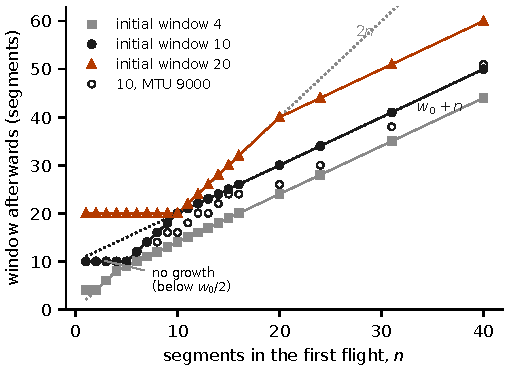
\includegraphics[width=\columnwidth]{fig_window}
\caption{Window after an $n$-segment flight on plain TCP.}
\label{fig:window}
\end{figure}

\section{A Refuted Explanation, and the Ticket}\label{sec:ticket}
\emph{Larger window.} Take ML-DSA-44 with a 14\,500-byte request. The ClientHello is five segments, so the window stays at 10 and the twelve-segment request flight costs a round trip. The model also put the ticket (4\,940 bytes) in the response flight, which then has twelve segments and costs a second one. Measured, the transaction paid only one (402\ms against 501\ms at 100\ms RTT). A larger window after the ClientHello would explain that. Loosening the rule by two segments (a choice made after seeing the data) removes the round trip of the request flight and brings the mean error to about 0.5\ms over \RN\ configurations. A test with predictions fixed in advance (222-byte response, so that only the client's flight can cost a round trip; request flights of 9--15 segments; \CN\ cells) refutes it (Table~\ref{tab:tests}). In Fig.~\ref{fig:stagec} (measured latency as circles, rule~(1) solid, the loosened rule dashed) the step is the extra round trip; it moves with the size of the ClientHello (2, 5, 6 and 8 segments), which sets the window of the request flight. Rule~(1) is right on all cells (mean error \CMaeZero\ms); the loosened rule is wrong by a round trip on \CWrongTwo. Table~\ref{tab:ablation} compares five models, each adding one element to the one above, by mean absolute error (MAE) and cells wrong by a round trip ($>$0.5 RTT), on the \AblFixedN\ resumed configurations and on the \AblCFixedN-cell client-window test, which separates only the window rules (\texttt{analyze\_\allowbreak l1\_\allowbreak model\_\allowbreak comparison.py}). A window fixed at $w_0$ is wrong on \AblCFixedOff\ of the \AblCFixedN\ client-window cells and textbook slow start on \AblCSlowOff, so the validation test is what the predictions need. The small flights of the resumed configurations cannot tell the first three models apart (\AblFixedOff, \AblSlowOff\ and \AblLinuxOff\ wrong); only the ticket timing fixes them (\AblEarlyOff).

\begin{table}[t]
\caption{What each part of the model adds (MAE in ms; cells wrong by a round trip).}
\label{tab:ablation}
\centering\footnotesize\setlength{\tabcolsep}{4pt}
\begin{tabular}{@{}lrrrr@{}}
\toprule
 & \multicolumn{2}{c}{\AblFixedN\ resumed} & \multicolumn{2}{c}{\AblCFixedN\ client window}\\
Model & MAE & wrong & MAE & wrong\\
\midrule
Window fixed at $w_0$ & \AblFixedMae & \AblFixedOff & \AblCFixedMae & \AblCFixedOff\\
Textbook slow start & \AblSlowMae & \AblSlowOff & \AblCSlowMae & \AblCSlowOff\\
+ Linux validation, rule (1) & \AblLinuxMae & \AblLinuxOff & \AblCLinuxMae & \AblCLinuxOff\\
+ OpenSSL write pattern, ticket joined & \AblJoinedMae & \AblJoinedOff & --- & ---\\
+ ticket written on the Finished & \AblEarlyMae & \AblEarlyOff & --- & ---\\
\bottomrule
\end{tabular}
\end{table}

\begin{figure}[t]
\centering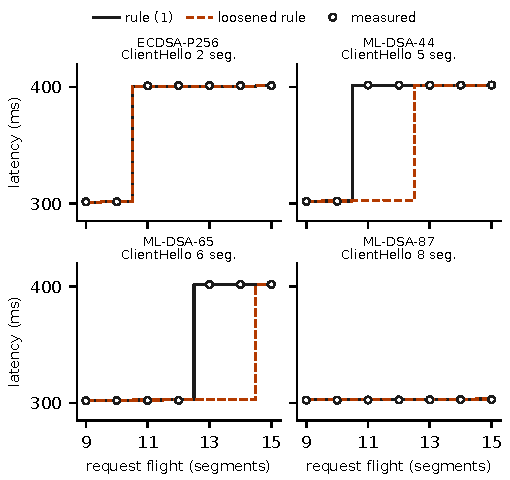
\includegraphics[width=\columnwidth]{fig_stagec}
\caption{Latency of a resumed transaction against the segments of the request flight.}
\label{fig:stagec}
\end{figure}

\emph{Ticket.} The remaining error sits on the server's side. The ticket embeds the client certificate (4 to 6 segments for ML-DSA-44, -65 and -87), and the model had joined it to the response flight (the joined-ticket model). Suppose instead that OpenSSL writes it separately as soon as the Finished arrives (the early-ticket model, Fig.~\ref{fig:ticket}). If the request flight needs an extra round trip, as for ML-DSA-44, the ticket is acknowledged by the time the response leaves and no longer occupies the window; if not, as for ML-DSA-65, the two share it. Others' data agree: the 15 server segment counts of Dubetskyy and Cano~\cite{dubetskyy2026} come out right only if the two NewSessionTicket messages and the close\_notify alert each leave as a segment of their own (5 of 5 combinations with three segments, none with 0, 1, 2 or 4; calculated after their numbers were published, \texttt{analyze\_dubetskyy\_segments.py}), although those connections did not resume. Removing the ticket fixes ML-DSA-44 but predicts ML-DSA-65 a round trip too fast (303 against 402\ms), so timing matters, not presence. The early-ticket model reproduces all \RN\ resumed configurations with a mean error of \REarlyMae\ms. A second test with predictions fixed in advance (\DN\ cells; requests of 302 and 19\,460 bytes; responses of 3--12 segments) has \DDiff\ cells where the two models differ by a round trip: the early ticket is right on all of them, the joined ticket on none (exact sign test $p=\SignDP$; Table~\ref{tab:tests}).

\emph{The server's window.} Both models are wrong on the same \DBothWrong\ cells (ML-DSA-44 and -65, a request that needs an extra round trip, responses of 11--12 segments): the server's window exceeded ten once the ticket was acknowledged, which (1) does not predict. A third test (\EN\ cells, responses of 10--18 segments) maps it. The largest response without an extra round trip is \EFitEcdsa, \EFitMlFourFour\ and \EFitMlSixFive\ segments for tickets of 1, 4 and 5 segments (ECDSA-P256, ML-DSA-44, -65). With different server and client algorithms the limit follows the client's certificate, hence the ticket, in \MixRight\ of \MixN\ pairs, a small sample (the exception: server ECDSA-P256, client ML-DSA-65, \MixFitExc\ against \MixPredExc). Nor is the window a property of the stack alone: in a \GenCells-cell scan (RTT \GenRttLo--\GenRttHi\ms, \GenRateLo--\GenRateHi\,Mbit/s, MTU \GenMtuLo--\GenMtuHi) the largest response without an extra round trip is \GenWMFourFourRttThirty\ and \GenWMSixFiveRttThirty\ segments for ML-DSA-44 and -65 at 30\ms, and \GenWMFourFourMtuLow\ for ML-DSA-44 at MTU~\GenMtuLo\ (ML-DSA-65 shows no step up to the largest response tested, \GenRespMax\ segments), whereas at 5\ms and at \GenRateLo\,Mbit/s every suite stays at \GenWEcRttFive. With server authentication only, where the ticket has one segment, the limit is \ServWindow\ for all three suites, and the early-ticket rule with a window of ten is wrong by a round trip in \ServWrong\ of \ServCells\ cells, as predicted before the measurement.

\emph{When the acknowledgment counts.} The order of the ticket's acknowledgment and the response does not decide the window. Captures on the server's link (\RaceN\ resumed transactions, ten networks) show at least one segment of the ticket acknowledged before the response is written in \RaceBeforePct\% of them, including those where the window stayed at ten. What separates the outcomes, a finding made afterwards, is when the last acknowledgment of the ticket arrives: the window exceeds ten segments when it comes more than \RaceThr\ms after the last request segment (\RaceRight\ of \RaceMlN\ ML-DSA transactions; exact 95\% interval \CiRaceLo--\CiRaceHi\%).

A request-size sweep with predictions committed beforehand confirmed the rule: outside a borderline band (cells whose median lies within 0.06\ms of the threshold), \RaceTwoRight\ of \RaceTwoScored\ cells had the predicted class (95\% Wilson interval [90, 100]\%), and the rule classified \RaceTwoOosRight\ of \RaceTwoOosN\ transactions ([97, 99.5]\%). It gives the direction of the effect, not the size of the window. The controls with a small request are all right (\ECtlWrong\ of \ECtlN\ cells wrong). The threshold is a local ordering at the server, in microseconds and unrelated to the RTT. On this machine the rule hardly depends on it (Table~\ref{tab:thr}: 97--99\% of the transactions from 0.04 to 0.10\ms, 94.5\% at 0.02\ms), but it does not carry over to the other machines (Section~\ref{sec:repl}). The table gives the share of observations in which ``the ACK arrives more than $T$ after the last request segment'' agrees with the outcome; $T=0.049$\ms was chosen on the first run, so the table is post hoc.

\emph{What the kernel does.} A function trace of the server's kernel (criterion in the analysis script, committed before the run) covers \KerN\ acknowledgments of the ticket. Reno examines every one, yet calls \texttt{tcp\_slow\_start} for none of the \KerBeforeN\ that arrive before the last request segment and for \KerAfterSS\% of the \KerAfterN\ that arrive after it. The rule classifies \KerRight\ of \KerN\ (\KerPct\%; exact interval \CiKerLo--\CiKerHi\%). The \KerWrong\ misses lie within \KerMissNear\ms of the threshold, about the resolution of the alignment of the two clocks.

A second run avoids the alignment problem by reading the sender's state at each acknowledgment (bpftrace probes on both functions; \StN\ acknowledgments, joined with the capture by port and acknowledgment number). \texttt{tcp\_\allowbreak slow\_\allowbreak start} is called iff the kernel's own test holds, i.e.\ \texttt{is\_\allowbreak cwnd\_\allowbreak limited} holds, or \texttt{snd\_\allowbreak cwnd} is below twice \texttt{max\_\allowbreak packets\_\allowbreak out} (\StPOneRight\ of \StPOneN, as registered). Two other registered criteria were not met. The burst of the response equals the window at the write minus the ticket segments still unacknowledged in \StPTwoPct\% of the transactions (criterion 90\%), and the 0.049\ms rule agrees with the state for \StPThreeRight\ of \StPThreeN\ acknowledgments near the threshold (\StPThreePct\%). The rule is a proxy, then, not the mechanism: the threshold was fixed after the first run (post hoc), predicts only on the machines where it was measured, and is not a constant of Linux TCP.

Looking at the data afterwards (post hoc), \StLateInflight\ of the \StLate\ acknowledgments that come more than 0.049\ms after the last request segment are processed with the response already in flight, where the test holds (median \texttt{packets\_out} \StAfterPk, against \StBeforePk\ for the others). Of the \StEarly\ acknowledgments up to 0.049\ms after it, \StEarlyLimited\ are limited, all of them ML-DSA-65, where \texttt{max\_packets\_out} reaches six and $10<2\times6$. A third group is more puzzling: the capture shows \StDeferredN\ acknowledgments before the write but more than 0.049\ms after the last request segment, and \StDeferred\ of them are processed after the write. The window follows from the last acknowledgment of the ticket: the burst of the response equals the window after it (\StPTwoBRight\ of \StPTwoBN\ within one segment).

\emph{Why the acknowledgments are late, and the intervention.} Two explanations for the delay were tested, and both failed. A third run (probes on the socket backlog; \BkN\ ticket acknowledgments) asked whether socket ownership explains it: Only \BkDef\ were processed from the backlog, and both registered criteria failed (\BkAPct\% and \BkBPct\% against 90\%). Afterwards we found that \texttt{tcp\_slow\_start} was called for all \PhAfterSS\ acknowledgments processed after the first write of the response returned, and for \PhBeforeSS\ of the \PhBefore\ processed before it (post hoc), most of them in softirq context. A fourth run (probes on the queueing to the CPU backlog, on the receive path and on the softirq; \HN\ ticket acknowledgments) asked whether they wait in the softirq queue, and failed its registered criteria too. Only \HAOne\ of the \HALate\ late acknowledgments (\HAPct\%) had been queued before the write returned (criterion 80\%), and the wait from queueing to processing was short (median \HWaitMed\,\textmu s, on the same CPU). Post hoc, they were queued a median \HEnqMed\,\textmu s after the write returned, although the capture shows them on the link 0.07\ms before it. Why they are queued late is not established.

An intervention, at least, settles the role of the ticket. When the server issues no ticket on resumed connections (predicted beforehand), the response burst is at most ten segments in all \NtkCells\ cells, including the \NtkEffect\ in which it exceeds ten with the ticket (exact sign test on those pairs $p=\SignNtkP$; with seven pairs no result can be smaller).

\begin{table}[t]
\caption{Robustness of the ticket-timing rule to its threshold $T$ (post hoc).}
\label{tab:thr}
\centering\small
\begin{tabular*}{\columnwidth}{@{\extracolsep{\fill}}p{0.30\columnwidth}rrrrrr@{}}
\toprule
$T$ (ms) & 0.02 & 0.04 & 0.049 & 0.06 & 0.08 & 0.10\\
\midrule
Burst $>10$, 399 transactions (\%) & 94.5 & 97.0 & 98.7 & 98.7 & 97.2 & 97.2\\
\texttt{tcp\_slow\_start} called, 799 ACKs (\%) & 93.4 & 94.1 & 95.6 & 96.5 & 96.7 & 96.5\\
\bottomrule
\end{tabular*}
\end{table}

\begin{figure}[t]
\centering
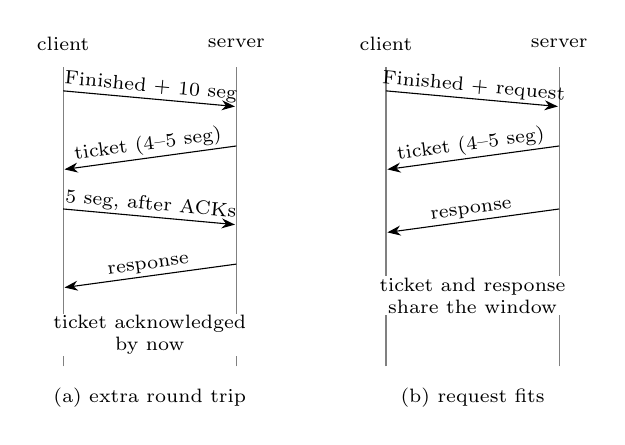
\begin{tikzpicture}[x=1mm,y=1mm,font=\scriptsize,>=Stealth,lab/.style={fill=white,inner sep=0.5pt},a/.style={->,shorten >=0.5pt}]
\foreach \o in {0,41}{\node at (\o,41) {client}; \node at (\o+22,41) {server}; \draw[gray] (\o,0) -- (\o,38); \draw[gray] (\o+22,0) -- (\o+22,38);}
% (a) the request flight needs an extra round trip
\draw[a] (0,35) -- node[above,sloped,inner sep=1pt] {Finished + 10 seg} (22,33);
\draw[a] (22,28) -- node[above,sloped,inner sep=1pt] {ticket (4--5 seg)} (0,25);
\draw[a] (0,20) -- node[above,sloped,inner sep=1pt] {5 seg, after ACKs} (22,18);
\draw[a] (22,13) -- node[above,sloped,inner sep=1pt] {response} (0,10);
\node[lab,align=center] at (11,4) {ticket acknowledged\\by now};
\node at (11,-4) {(a) extra round trip};
% (b) the request fits in the window
\draw[a] (41,35) -- node[above,sloped,inner sep=1pt] {Finished + request} (63,33);
\draw[a] (63,28) -- node[above,sloped,inner sep=1pt] {ticket (4--5 seg)} (41,25);
\draw[a] (63,20) -- node[above,sloped,inner sep=1pt] {response} (41,17);
\node[lab,align=center] at (52,9) {ticket and response\\share the window};
\node at (52,-4) {(b) request fits};
\end{tikzpicture}
\caption{Ticket timing. (a) The request flight needs an extra round trip. (b) It does not.}
\label{fig:ticket}
\end{figure}

\begin{table}[t]
\caption{Pre-registered tests and outcomes.}
\label{tab:tests}
\centering\footnotesize\setlength{\tabcolsep}{3pt}
\begin{tabular}{@{}r>{\raggedright\arraybackslash}p{0.43\columnwidth}>{\raggedright\arraybackslash}p{0.21\columnwidth}>{\raggedright\arraybackslash}p{0.22\columnwidth}@{}}
\toprule
 & Test and rule & Criterion & Result\\
\midrule
1 & Client window: validated rule & none wrong & \CWrongZero\ of \CN\ (met)\\
2 & Client window: loosened by 2 segments & none wrong & \CWrongTwo\ of \CN\ (refuted)\\
3 & Ticket joined with response, discriminating cells & none wrong & \DJoinedWrongDiff\ of \DDiff\ (refuted)\\
4 & Ticket written on Finished, discriminating cells & none wrong & \DEarlyWrongDiff\ of \DDiff\ (met)\\
5 & Ticket written on Finished, all cells & none wrong & \DEarlyWrong\ of \DN\\
6 & Request-size sweep, ticket-timing rule, cells outside the borderline band & predicted class & \RaceTwoRight\ of \RaceTwoScored\ (met)\\
7 & Kernel trace, acknowledgments of the ticket & rule classifies & \KerRight\ of \KerN\ (\KerPct\%)\\
8 & State trace: \texttt{tcp\_slow\_start} iff the kernel's test holds & as registered & \StPOneRight\ of \StPOneN\ (met)\\
9 & State trace: response burst equals the window at the write minus unacknowledged ticket segments & 90\% of transactions & \StPTwoPct\% (not met)\\
10 & Socket backlog explains the delay & 90\% & \BkAPct\% and \BkBPct\% (not met)\\
11 & Softirq queue explains the delay & 80\% of late acknowledgments & \HAPct\% (not met)\\
12 & No ticket issued: response burst $\le10$ segments & all cells & \NtkCells\ of \NtkCells\ (met)\\
13 & Rows 1--5 repeated on OpenSSL 4.1.0 and 3.6.5, same machine, 3.5 as baseline (criteria G1--G4) & all four met & \GxFourMet\ (4.1.0) and \GxThreeMet\ (3.6.5) of 4 (met)\\
14 & Rows 1--5 and the ticket position on Go \texttt{crypto/tls} (criteria H1--H5) & all five met & \GoMet\ of 5 (not met: H1, H5)\\
15 & Window after a short flight under BBR and under fq pacing, plain TCP (criteria Q1--Q5) & all met & \GelevenMet\ of \GelevenN\ (met)\\
16 & Ticket timing on new cells: RTT 30 and 200\ms, requests of 302--19\,460\,B, OpenSSL~3.5 (criteria K1--K4 per RTT) & all met & \GtwelveMet\ of \GtwelveK\ (met)\\
17 & Client-window and ticket-timing tests under BBR (criteria B1--B5) & all met & \GfBbrMet\ of \GfBbrK\ (met)\\
18 & The same tests with delayed acknowledgments (criteria D1--D5) & all met & \GfDelMet\ of \GfDelK\ (met)\\
19 & Window rule under loss of 0.1, 0.5 and 1\%, plain TCP (criteria L1--L3) & all met & \GsixMet\ of \GsixK\ (not met: L1)\\
\bottomrule
\end{tabular}
\end{table}

\section{Does It Replicate?}\label{sec:repl}
We repeated the plain-TCP test (stage~A, four configurations, ten repetitions) on four kernels of the i7-5600U (6.8, 6.14, 6.17, 7.0), on an i9-10900K (7.0.0-42, two runs) and on an Arm machine (ASUS Ascent GX10 with an NVIDIA GB10: Cortex-X925 and A725, 6.14 and 7.0). In all eight runs rule~(1) is exact in the base, MTU 1\,280 and $w_0=20$ configurations. At MTU~9\,000 only 35--40\% of the flight sizes match, on every machine alike, so that deviation belongs to the jumbo-frame path (the receive window, Section~\ref{sec:window}), not to a kernel or a CPU. Table~\ref{tab:repl} gives, per platform, the share of flight sizes with the exact window at MTU~9\,000 and the results of the ticket tests: the state test (\texttt{tcp\_\allowbreak slow\_\allowbreak start} iff the sender is limited), the cells with a burst of at most ten segments when no ticket is issued, and the share of ticket acknowledgments processed from the socket backlog (``--'': not run).

The ticket tests ran on the i7-5600U (7.0) and on the Arm machine (6.14 and 7.0), and most of their results carry over. \texttt{tcp\_slow\_start} is called iff the kernel's test holds for 815 of 815 acknowledgments (6.14) and 817 of 817 (7.0). Without a ticket the response burst is at most ten segments in all 18 cells; the ticket changes two of them on Arm, on both kernels, and seven on the i7. The two queue explanations fail again. Only 4.8\% (6.14) and 5.0\% (7.0) of the ticket acknowledgments are processed from the socket backlog (35.4\% on the i7), and only 5 of 339 and 14 of 337 after the write returned (117 of 331 on the i7). Two registered criteria split by machine: the burst criterion is met on Arm (99.2\% and 98.7\%, against 89.8\% on the i7) and the threshold criterion is not (79.4\% and 77.9\%, against 68.9\%), so the 0.049\ms rule stays a proxy.

\begin{table}[t]
\caption{Replication on other kernels and CPUs.}
\label{tab:repl}
\centering\footnotesize\setlength{\tabcolsep}{3pt}
\begin{tabular*}{\columnwidth}{@{\extracolsep{\fill}}lcccc@{}}
\toprule
Platform, kernel & MTU 9\,000 & state & no ticket & backlog\\
\midrule
i7-5600U, 6.8 / 6.14 / 6.17 & 35 / 40 / 35\% & -- & -- & --\\
i7-5600U, 7.0 & 35\% & 799/799 & 18/18 & 35.4\%\\
i9-10900K, 7.0 (2 runs) & 35\% & -- & -- & --\\
Arm GX10, 6.14 & 40\% & 815/815 & 18/18 & 4.8\%\\
Arm GX10, 7.0 & 35\% & 817/817 & 18/18 & 5.0\%\\
\bottomrule
\end{tabular*}
\end{table}

\section{Other Releases, a Second Library and Other Controllers}\label{sec:other}
\emph{OpenSSL releases.} The code that writes the ticket does not change across the releases we measured. The server's transition after the client's Finished, the flush after the ticket is built and the construction of the ticket are textually identical in 3.5.4, 3.5.9 and 3.6.5; in 4.1.0 the order is unchanged too (it adds DTLS~1.3 acknowledgments and moves the test of whether to send a ticket into the transition; \texttt{audit\_ossl\_ticket\_path.py}). Full handshakes agree with 3.5.4 in \OvTwoSame, \OvThreeSame\ and \OvFourSame\ of \OvTwoAll\ configurations for 3.5.9, 3.6.5 and 4.1.0, and the rest differ by at most one segment. Reading is not measuring, so we repeated the \CN\ client-window cells and the \DN\ ticket-timing cells on 3.6.5 and 4.1.0, with 3.5 as a baseline on the same machine (row 13 of Table~\ref{tab:tests}; predictions and criteria fixed before the run). All four criteria were met on both releases. On both, the validated rule was wrong on \GxFourCWrong\ of the \CN\ client-window cells and the rule loosened by two segments on \GxFourCLoose; among the \DDiff\ discriminating cells the early-ticket model was wrong on \GxFourDisEarly\ and the joined-ticket model on \GxFourDisJoined, and the resumed latencies differ from those of 3.5 by at most \GxMaxDiff\ms.

\emph{A second library.} Go's \texttt{crypto/tls} writes the ticket with the server's first flight on a resumed connection and keeps the client's certificates in it (tickets of 1.8 to 16\,KB). Its ClientHello, which carries the ticket and with it the certificates, is 2, 8, 10 and 13 segments for the four suites (OpenSSL: 2, 5, 6, 8), so the sizes and positions of the writes differ from OpenSSL's. We took them from a calibration run of Go's own probe, left the model unchanged and repeated the two tests (row 14 of Table~\ref{tab:tests}; one machine). Of the five registered criteria, \GoMet\ were met. The first-flight ticket model was wrong on \GoDisGoWrong\ of the \GoDisN\ cells where it differs from the joined-ticket model (which was wrong on all of them) and on \GoWrongAll\ of \GoDN\ cells in all; the loosened rule and textbook slow start were refuted. Two criteria failed. Rule~(1) was wrong on \GoCWrong\ of \GoCN\ client-window cells, where at most two were allowed, and the byte check failed because the client also reads a 24-byte \texttt{close\_notify} that the calibration lacks (it passes with that allowance, which we had not registered).

All \GoWrongSuiteN\ wrong cells are ML-DSA-87, and all are a round trip faster than predicted. A packet capture shows why. The ML-DSA-87 first flight (13 segments) exceeds the window of ten, and the client sends its Finished and request after the first ten: the tail of the flight is the end of the ticket, which it need not wait for. Our model treats a flight as complete before the next step. A variant that stops charging for the tail, formulated after seeing the data, brings the wrong cells from \GoPostBefore\ to \GoPostAfter. The position and size of the ticket do depend on the library, then, and the model follows them once they are measured, but it has a limit of its own where a flight is longer than the window.

\emph{Other controllers and pacing.} On plain TCP (stage~A, one machine; row 15 of Table~\ref{tab:tests}), with hypotheses read from the kernel source before the run, all \GelevenN\ criteria were met. Under BBR (the in-tree v1) the window after an $n$-segment flight is $w_0+n$ for every $n$, because its update adds the packets acknowledged without testing whether the sender was limited; rule~(1) is wrong for all nine sizes $n\le9$. Under fq pacing with Reno or Cubic the window is that of (1) (one of 20 sizes differs, by two segments, for Cubic at $n=40$), and a flight within the initial quantum takes as long as on the unpaced baseline.

\emph{The ticket tests under BBR and delayed acknowledgments.} Both were repeated with predictions and criteria fixed in advance (rows 17 and 18; one machine, RTT 100\ms). Under BBR the model with window $w_0+n$ was wrong on \GfBbrCWrong\ of \GfBbrCN\ client-window cells and rule~(1) on all \GfBbrRuleWrong\ where the two differ; in the ticket-timing cells the BBR model was wrong on \GfBbrDWrong\ of \GfBbrDN\ and the model of this paper on \GfBbrRenoWrong\ of the \GfBbrDDiff\ cells where they differ. All \GfBbrK\ criteria were met, narrowly in stage~D: on the other two of those cells (ML-DSA-87) the measurement lies between the models, 54\ms above BBR's prediction and 45\ms below Reno's, so they favour neither, and one ECDSA cell is 82\ms below both. With delayed acknowledgments rule~(1) was wrong on \GfDelCWrong\ of \GfDelCN\ cells and the early-ticket model on \GfDelEarlyAll\ of \GfDelDN\ (the joined-ticket model on \GfDelJoinedDiff\ of the \GfDelDDiff\ discriminating cells); all \GfDelK\ criteria were met.

\emph{Ticket timing on new cells.} The ticket hypothesis was found on \DDiff\ discriminating cells at one RTT (95\% Wilson interval of the success rate [72, 100]\%), so it needed a test elsewhere. We ran it at RTT 30 and 200\ms with requests of 302 to 19\,460\,B (OpenSSL~3.5, one machine, row 16; \GtwelveCells\ cells, \GtwelveDis\ discriminating; predictions and criteria fixed before the run). All \GtwelveK\ criteria were met: the early-ticket model was wrong on \GtwelveEarlyDis\ of the discriminating cells and the joined-ticket model on \GtwelveJoinedDis\ (interval [\GtwelveWilsonLo, 100]\%). Over all \GtwelveCells\ cells the early-ticket model was wrong on \GtwelveEarlyAll, the same cell at both RTTs (ML-DSA-65, 19\,460-byte request, response of 14 segments), where it charges a round trip that was not paid.

\section{Recommendations and Limits}
Five recommendations follow. They hold for the tested stack (Linux 7.0, Reno, OpenSSL~3.5; 3.6.5 and 4.1.0 in the ticket tests). The first, second and fifth rest on (1), the window of Reno and Cubic (under BBR it is $w_0+n$, row 15 of Table~\ref{tab:tests}), the third and fourth on the ticket tests.
\begin{enumerate}
\item \emph{Budget each direction and each write in segments of the actual MSS.} A flight costs a round trip when it exceeds the window that the previous flight in the same direction left. Compute that window with (1), not with $w_0$, and count tickets and every other separate write.
\item \emph{Treat the size of the ClientHello as a threshold.} With $w_0=10$, five segments leave the window at 10 and six raise it to 12, so a few bytes (a ticket, a larger key share) can lift the next client flight across the window and save a round trip (a larger key share would act the same way, but we did not measure it). Compute the segment count; a larger ClientHello is not necessarily a costlier one.
\item \emph{After a ticket, budget the response flight at ten segments.} Ticket and response share the window if the request fits; if it needs an extra round trip, the ticket's acknowledgment can enlarge the server's window to 11--15 segments. Ten was pessimistic in the \DBothWrong\ cells where it was wrong.
\item \emph{Measure the server's window on the actual path.} After a ticket it is the window after every acknowledgment of the ticket that the kernel processes while the sender is limited, which depends on RTT, rate, MTU and on when the server's acknowledgments are processed; no rule here predicts it from the network.
\item \emph{Repeat the plain-TCP test on each kernel and TLS library before relying on (1).} Before using jumbo frames, check that the receive buffer holds the flight: otherwise the sender is not window-limited and (1) does not apply.
\end{enumerate}

\emph{Limits: scope of the measurements.} The window rule was tested on seven machine-kernel combinations (eight runs), the ticket tests of Table~\ref{tab:repl} on two machines (three runs) and those of Section~\ref{sec:other} on one. The link is emulated (two network namespaces and \texttt{tc netem}); loss was tested on plain TCP only, and cross traffic, RTT variation and a real path not at all. Each measurement used one connection at a time, so the processing of acknowledgments under concurrent load is untested, and CPU and throughput are not studied. The transactions use mutual authentication, 30 per cell (too few for tails), and Reno or Cubic, which give the same window at these sizes. At MTU~9\,000 the rule holds only when the receive buffer does not limit the sender (Section~\ref{sec:window}), and four flight sizes stay below it even then; record splitting at that MTU and the full handshakes there are treated in the companion paper~\cite{paperone}.\par\emph{Limits: the TLS library.} We used two TLS libraries: OpenSSL (three releases that share the code writing the ticket) and Go's \texttt{crypto/tls} on one machine. The window rule and the processing of acknowledgments are Linux's; writing the ticket when the Finished arrives and cutting data into 16-KB record writes are OpenSSL's. The source of GnuTLS 3.8.14 and of wolfSSL 5.9.4 (read, not measured) also writes the ticket after the client's Finished, but GnuTLS issues two tickets that each hold the client's certificates and wolfSSL stores no ML-DSA certificate in its ticket (it exceeds 2\,048 bytes), so the size and the number of tickets, not only their position, depend on the library.

\section{Conclusion}
A few bytes can decide a round trip. With an initial window of ten, five ClientHello segments leave the window where it was and six lift it by two, because Linux adds a segment per acknowledgment only while the sender is limited. That inequality explains most of what our model had missed, not all: the last two transactions led us to the session ticket, which OpenSSL writes by itself and whose acknowledgment can enlarge the server's window by several segments. Predictions fixed in advance refuted the larger client window, whereas the explanations we tried for the late acknowledgments (the socket backlog, the softirq queue) failed their criteria.

Three limits shape what a reader can take away. The rule is Reno's and Cubic's, since BBR leaves $w_0+n$; under loss it holds for every connection without a retransmission. The ticket's position and size depend on the library, as Go shows. And the server's window after a ticket still has no formula. A practitioner can budget flights with (1) and the five recommendations, then measure the response flight on the real path. We explain one component of the latency of post-quantum TLS, the extra round trips, not the cost of deploying it. A researcher is left with a sharper question: why does the kernel process those acknowledgments late?

\emph{Acknowledgments.} This work was supported by the Intelligently Connected Networks LABoratory (PTIT) and the Banking Academy of Vietnam. 
\par During the preparation of this work, the first author used ChatGPT (OpenAI) and Claude (Anthropic) to assist with routine analysis scripting, language editing, and consistency checks. After using these tools, both authors reviewed, validated, and edited the code and content as needed, and take full responsibility for the content of the published article.
\par\emph{Availability.} Scripts, measurement files, the pre-registered predictions with commit times and tables derived from the kernel traces are on Zenodo: doi:\allowbreak10.5281/\allowbreak zenodo.\allowbreak24355942 (all versions) and doi:\allowbreak10.5281/\allowbreak zenodo.\allowbreak24355943 (version l1-v1.0). The raw traces and captures of the ticket tests (98\,MB compressed) are doi:\allowbreak10.5281/\allowbreak zenodo.\allowbreak24384873.

\bibliographystyle{ACM-Reference-Format}
\bibliography{refs}
\end{document}
